% =============================================================================
% Virtual Element Method for oral biofilm mechanics:
% from confocal images to viscoelastic fracture on arbitrary polygonal meshes
%
% Target: Computational Mechanics (Springer)
% Authors: Nishioka K., Aldakheel F., Wriggers P.
% Affiliation: Institute of Continuum Mechanics (IKM),
%              Leibniz Universität Hannover, Germany
% =============================================================================
\documentclass[smallextended]{svjour3}
\smartqed
\usepackage{amsmath,amssymb,bm}
\usepackage{graphicx}
\usepackage{booktabs}
\usepackage{hyperref}
\usepackage{xcolor}
\usepackage{enumitem}
\usepackage{multirow}
% Draft layout — remove before submission to use journal defaults
\usepackage[a4paper, margin=25mm, top=20mm, bottom=20mm]{geometry}
\setlength{\parskip}{0pt}
\setlength{\floatsep}{8pt plus 2pt minus 2pt}
\setlength{\textfloatsep}{10pt plus 2pt minus 2pt}
\setlength{\intextsep}{8pt plus 2pt minus 2pt}
\setlength{\abovecaptionskip}{4pt}
\setlength{\belowcaptionskip}{2pt}

\graphicspath{{results/paper_vem/}}

% Notation
\newcommand{\vect}[1]{\bm{#1}}
\newcommand{\mat}[1]{\mathbf{#1}}
\renewcommand{\tens}[1]{\boldsymbol{#1}}
\newcommand{\dd}{\mathrm{d}}
\newcommand{\DI}{\mathrm{DI}}
\newcommand{\tr}{\mathrm{tr}}
\DeclareMathOperator{\diag}{diag}
% Phase-field damage variable (distinct from spatial dimension d)
\newcommand{\pf}{\varphi}

\journalname{Computational Mechanics}

\begin{document}

\title{Virtual Element Method for oral biofilm mechanics:
from confocal images to viscoelastic fracture
on arbitrary polygonal meshes}
\titlerunning{VEM for oral biofilm mechanics}

%\author{Keisuke Nishioka \and Fadi Aldakheel \and Peter Wriggers}
\author{Keisuke Nishioka}

%\institute{K.~Nishioka \and F.~Aldakheel \and P.~Wriggers \at
\institute{K.~Nishioka \at
  Institute of Continuum Mechanics (IKM), \\
  Leibniz Universit\"at Hannover, \\
  Appelstra\ss e 11, 30167 Hannover, Germany \\
  \email{nishioka@ikm.uni-hannover.de}
}

\date{Received: date / Accepted: date}

\maketitle

% =====================================================================
\begin{abstract}
Oral biofilms are structured multispecies communities whose mechanical
properties depend on microbial composition.
We present a Virtual Element Method (VEM) framework that reduces the
image-to-mechanics pipeline from five steps (confocal segmentation,
voxelisation, marching cubes, tetrahedral meshing, FEM) to two
(Voronoi tessellation from colony detection, VEM solve).
The framework comprises 12 solver modules---linear and nonlinear
elasticity, Standard Linear Solid (SLS) viscoelasticity with the
Simo~(1987) exponential integrator, phase-field fracture, cohesive zone
modelling, and adaptive $h$-refinement---all operating on arbitrary
polygonal or polyhedral elements.
Material properties are assigned per colony via a composition-based
Diversity Index (DI) derived from TMCMC-calibrated species dynamics,
yielding DI-dependent stiffness $E(\DI)$, fracture toughness $G_c(\DI)$,
and SLS relaxation parameters.
The viscoelastic VEM reproduces analytical solutions for uniform strain
fields to machine precision (relative error $1.3\times10^{-15}$), and
achieves $L^2$ convergence rate $2.16$ on Voronoi meshes for
non-uniform manufactured solutions (vs.\ $1.88$ for P$_1$ FEM on
triangles; $H^1$ rates: VEM~$1.31$ vs.\ FEM~$0.99$).
Growth-coupled simulations on 30-cell meshes over 50 macro time steps
reveal divergent mechanical evolution:
commensal biofilms stiffen ($E_\infty$: $392\to847$\,Pa,
$\DI$: $0.382\to0.090$) while
dysbiotic biofilms soften ($E_\infty$: $376\to153$\,Pa,
$\DI$: $0.396\to0.623$) under comparable initial conditions.
A CNN-accelerated variant replaces colony detection and VEM solving
with a U-Net (confocal $\to$ DI map) and surrogate network
(DI $\to$ displacement), achieving $>100\times$ speedup for real-time
applicability.
To our knowledge, this is the first application of VEM to biofilm
mechanics.
\end{abstract}

\keywords{Virtual Element Method \and biofilm mechanics \and
viscoelasticity \and phase-field fracture \and
composition-dependent properties \and confocal imaging \and
deep learning surrogate}

% =====================================================================
\section{Introduction}
\label{sec:intro}

Oral biofilms are structured multispecies communities that colonise tooth
surfaces, forming a mechanically significant interface between the
tooth substrate and the oral cavity~\cite{Flemming2010}.
The transition from a healthy (commensal) to a disease-associated
(dysbiotic) state is driven by shifts in species
composition~\cite{Heine2025}, which in turn affect the biofilm's
elastic modulus~\cite{Pattem2018,Pattem2021}, viscoelastic relaxation
behaviour~\cite{Peterson2015,Stoodley1999}, and fracture
toughness~\cite{Gloag2020a,Gloag2020b}.
Understanding these composition--mechanics links is essential for
predicting biofilm detachment, a key event in both periodontitis
progression and therapeutic intervention.

Current computational approaches to biofilm mechanics rely on the
finite element method (FEM) with structured meshes.
Klempt et al.~\cite{Klempt2024} demonstrated staggered coupling of
species dynamics with continuum mechanics on a conformal tetrahedral
mesh.
However, the mesh generation pipeline (confocal image $\to$ voxel
segmentation $\to$ marching cubes $\to$ tetrahedral mesh $\to$ Abaqus
input) involves five labour-intensive steps, and standard FEM mesh
generators cannot naturally accommodate the arbitrary colony shapes
observed in confocal images.

The Virtual Element Method
(VEM)~\cite{BeiraodaVeiga2013,BeiraodaVeiga2014} offers a compelling
alternative.
As a generalisation of FEM, VEM solves partial differential equations
on meshes of \emph{arbitrary polygonal or polyhedral elements},
eliminating the need for standard element topologies.
The key innovation is the \emph{elliptic projection}
$\Pi^\nabla$ that maps \emph{virtual} (implicitly defined)
basis functions onto a polynomial subspace, from which the
stiffness matrix is assembled without ever constructing
explicit shape functions~\cite{Sutton2017}.

The VEM has been extensively developed for solid mechanics:
Gain et al.~\cite{Gain2014} formulated 3D VEM on polyhedral meshes,
Chi et al.~\cite{Chi2017} extended VEM to finite deformations,
and Antonietti et al.~\cite{Antonietti2022} reviewed higher-order
conforming formulations.
At IKM Hannover,
Wriggers and Hudobivnik~\cite{Wriggers2019} developed low-order 3D
VEM for elastoplasticity,
Aldakheel et al.~\cite{Aldakheel2018} introduced phase-field brittle
fracture on VEM meshes, and
Artioli et al.~\cite{Artioli2017} formulated inelastic VEM for
arbitrary-order polygonal meshes.
The comprehensive monograph~\cite{Wriggers2024} covers applications
from linear elasticity to contact mechanics.

For biofilm mechanics, VEM offers three specific advantages
(Fig.~\ref{fig:vem_schematic}):
\begin{enumerate}[nosep]
  \item \textbf{Mesh--image compatibility}: Voronoi tessellation from
    colony centroids yields a mesh where each cell corresponds 1:1
    to a micro-colony, enabling a 2-step pipeline
    (Fig.~\ref{fig:pipeline}).
  \item \textbf{Per-colony material assignment}: Each element receives
    its own composition-dependent material parameters without
    sub-element averaging.
  \item \textbf{Topology tolerance}: Growth, detachment, and crack
    propagation change the domain topology; VEM handles arbitrary
    element shapes without global remeshing.
\end{enumerate}

This paper presents a VEM framework for biofilm mechanics.
The principal contributions are:
\begin{enumerate}[nosep]
  \item[(i)] A viscoelastic VEM coupling the Simo~\cite{Simo1987}
    exponential integrator with VEM projection operators,
    validated for both uniform (machine-precision) and non-uniform
    ($L^2$ rate~2.16) strain fields in 2D.
  \item[(ii)] Composition-dependent constitutive laws that map a
    Diversity Index (DI) to stiffness $E(\DI)$, fracture toughness
    $G_c(\DI)$, and SLS relaxation parameters.
    We explicitly identify which mappings are experimentally
    supported and which remain assumptions
    (Section~\ref{sec:constitutive}).
  \item[(iii)] A growth-coupled VE-VEM demonstrating divergent
    mechanical evolution of commensal vs.\ dysbiotic biofilms,
    with quantitative computational cost comparison against FEM.
  \item[(iv)] A CNN-accelerated pipeline (U-Net + VEM surrogate)
    trained on 239 real CLASI-FISH confocal images from 14 donors,
    achieving $>100\times$ speedup over the traditional VEM workflow.
\end{enumerate}

The remainder is organised as follows.
Section~\ref{sec:math} introduces the mathematical framework.
Section~\ref{sec:constitutive} details the DI-dependent constitutive
laws, clearly distinguishing experimental support from modelling
assumptions.
Section~\ref{sec:pipeline} presents the confocal-to-VEM pipeline.
Section~\ref{sec:verification} provides numerical verification
including non-uniform benchmarks and computational cost comparisons.
Section~\ref{sec:applications} demonstrates biofilm applications.
Sections~\ref{sec:discussion}--\ref{sec:conclusions} discuss
limitations and conclusions.

% =====================================================================
\section{Mathematical framework}
\label{sec:math}

\subsection{VEM for linear elasticity}
\label{sec:vem:lin}

Consider a domain $\Omega \subset \mathbb{R}^{n_d}$ ($n_d=2,3$)
decomposed into a mesh $\mathcal{T}_h$ of non-overlapping polygonal
($n_d{=}2$) or polyhedral ($n_d{=}3$) elements~$E$.
Throughout, we adopt the Poisson ratio $\nu = 0.45$, reflecting
the nearly incompressible, hydrated nature of
biofilms~\cite{Peterson2015,Stoodley1999}.
For the lowest-order case ($k{=}1$), the local virtual element space on
element~$E$ with $n_v$ vertices is
\begin{equation}
  V_h^E = \bigl\{\, \vect{v}_h \in [H^1(E)]^{n_d} \;:\;
    \vect{v}_h|_{\partial E} \text{ piecewise linear},\;
    \Delta \vect{v}_h = \vect{0} \;\text{in } E
  \,\bigr\},
  \label{eq:vem_space}
\end{equation}
with degrees of freedom $\{\vect{u}_i\}_{i=1}^{n_v}$ at the vertices,
giving $n_\mathrm{dof}^E = n_d \cdot n_v$.

The elliptic projection
$\Pi^\nabla : V_h^E \to [\mathcal{P}_k(E)]^{n_d}$
minimises $a^E(\vect{v}_h - \Pi^\nabla \vect{v}_h, \vect{p})$
for all $\vect{p} \in [\mathcal{P}_k]^{n_d}$,
where $a^E(\cdot,\cdot)$ is the element bilinear form
(Fig.~\ref{fig:vem_schematic}).
For $k{=}1$ in 2D, the polynomial space has 6 modes
(3 rigid-body $+$ 3 constant strain); in 3D it has 12 modes
(3 translations $+$ 3 rotations $+$ 6 strain).

The projection is computed from the matrices
$\mat{G} = \mat{B}\,\mat{D}$ and
$\Pi^\nabla = \mat{G}^{-1}\,\mat{B}$,
where $\mat{D}$ evaluates polynomials at vertex DOFs and
$\mat{B}$ encodes the bilinear form via edge (2D) or face (3D)
integrals~\cite{Sutton2017}.
The element stiffness matrix decomposes as
\begin{equation}
  \mat{K}^E = \mat{K}^E_\pi + \mat{K}^E_\mathrm{stab},
  \label{eq:K_decomp}
\end{equation}
where $\mat{K}^E_\pi = (\Pi^\nabla)^\top \tilde{\mat{C}}\, \Pi^\nabla$
provides consistency and
$\mat{K}^E_\mathrm{stab} = \alpha_s\,\tr(\mat{C})\,|E|\,
(\mat{I} - \Pi^\nabla\mat{D})^\top(\mat{I} - \Pi^\nabla\mat{D})$
provides stability.
The stabilisation parameter $\alpha_s = 1.0$ follows the standard
IKM recipe~\cite{Wriggers2019,BeiraodaVeiga2013}; a sensitivity study
(Section~\ref{sec:alpha_s}) confirms that results are insensitive to
$\alpha_s \in [0.1, 1.0]$ for the mesh topologies used here.

\begin{figure}[t]
  \centering
  
\includegraphics[width=0.85\linewidth]{fig02_vem_schematic.pdf}
  \caption{VEM schematic: the elliptic projection $\Pi^\nabla$ maps
  virtual basis functions (defined implicitly on arbitrary polygons)
  onto a polynomial subspace, from which the stiffness matrix is
  assembled via consistency $\mat{K}_\pi$ and stabilisation
  $\mat{K}_\mathrm{stab}$ contributions.}
  \label{fig:vem_schematic}
\end{figure}

\subsection{Second-order (P$_2$) VEM}
\label{sec:vem:p2}

The $k{=}2$ extension places DOFs at both vertices and edge midpoints,
yielding $n_\mathrm{dof}^E = n_d(n_v + n_e)$ per element.
The polynomial basis expands to 12 modes in 2D
(3~rigid body $+$ 3~linear strain $+$ 6~quadratic).
Strain energy is evaluated by sub-triangulation with Gauss quadrature,
and a volume correction accounts for
$\mathrm{div}(\tens{\sigma}(\vect{p}_\alpha)) \neq \vect{0}$
in quadratic polynomial modes.
P$_2$ VEM achieves 15--45\% lower stress error than P$_1$ at the same
mesh size (see Section~\ref{sec:p1p2}).

\subsection{Viscoelastic VEM with the Simo integrator}
\label{sec:vem:ve}

We adopt the Standard Linear Solid (SLS / Zener) model with
DI-dependent parameters (Section~\ref{sec:constitutive}):
\begin{equation}
  \tens{\sigma}(t) = \mat{C}_\infty \tens{\varepsilon}(t) + \vect{h}(t),
  \label{eq:sls_stress}
\end{equation}
where $\mat{C}_\infty$ and $\mat{C}_1 = \mat{C}_0 - \mat{C}_\infty$
are the equilibrium and overstress constitutive matrices, and
$\vect{h}$ is the internal viscous stress satisfying
\begin{equation}
  \dot{\vect{h}} = \mat{C}_1\,\dot{\tens{\varepsilon}} - \vect{h}/\tau.
  \label{eq:h_ode}
\end{equation}
Following Simo~\cite{Simo1987}, Eq.~\eqref{eq:h_ode} is integrated
exactly over a time step $\Delta t = t_{n+1} - t_n$:
\begin{equation}
  \vect{h}_{n+1} = e^{-\Delta t/\tau}\,\vect{h}_n
  + \gamma\,\mat{C}_1\,\Delta\tens{\varepsilon},
  \qquad
  \gamma = \frac{\tau}{\Delta t}\bigl(1 - e^{-\Delta t/\tau}\bigr).
  \label{eq:simo_update}
\end{equation}
The algorithmic tangent modulus is
$\mat{C}_\mathrm{alg} = \mat{C}_\infty + \gamma\,\mat{C}_1$,
which enters the VEM stiffness as
\begin{equation}
  \mat{K}_\mathrm{alg}^E
  = (\tens{\Pi}_\varepsilon^E)^\top\,
    \mat{C}_\mathrm{alg}^E\,|E|\,
    \tens{\Pi}_\varepsilon^E
  + \mat{K}_\mathrm{stab}^E,
  \label{eq:K_alg}
\end{equation}
where $\tens{\Pi}_\varepsilon^E$ is the strain projector
($3 \times 2n_v$ in 2D, $6 \times 3n_v$ in 3D).
At each time step, the right-hand side includes the viscous
pre-stress contribution
$\vect{f}_h^E = -(\tens{\Pi}_\varepsilon^E)^\top\,|E|\,
e^{-\Delta t/\tau}\,\vect{h}_n^E$.

This formulation is \emph{unconditionally stable} for any $\Delta t > 0$
and exact for constant strain rate within a time step.

\begin{remark}[Machine precision for uniform strain]
\label{rem:machprec}
For $k{=}1$ VEM under uniform strain (e.g., confined compression),
the projection $\Pi^\nabla$ is exact and the stabilisation term
vanishes.
Consequently, the VEM solution coincides with the analytical
solution to machine precision.
This is a necessary (but not sufficient) condition for implementation
correctness.
Section~\ref{sec:nonuniform} presents non-uniform benchmarks that
test the interplay between projection error, stabilisation, and time
integration.
\end{remark}

\subsection{Extension to 3D polyhedral elements}
\label{sec:vem:3d}

The 2D formulation extends to polyhedral elements following
Wriggers et al.~\cite{Wriggers2019,Wriggers2024} and
Gain et al.~\cite{Gain2014}.
On a polyhedron~$E$ with $n_v$ vertices and $n_f$ faces,
the polynomial basis has 12 modes
(3~translations, 3~rotations, 6~constant strain),
giving $n_\mathrm{dof}^E = 3 n_v$.
The $\mat{B}$ matrix ($12 \times 3n_v$) is assembled via
face integrals using the midpoint rule on triangulated faces.
The strain projector
$\tens{\Pi}_\varepsilon$ ($6 \times 3n_v$) extracts rows 7--12
from the full projector, and the algorithmic tangent uses
$6 \times 6$ Voigt matrices for the isotropic SLS model.

\subsection{Neo-Hookean VEM for large deformations}
\label{sec:vem:nh}

For completeness, we include a hyperelastic Neo-Hookean
formulation following Chi et al.~\cite{Chi2017}:
\begin{equation}
  W(\mat{F}) = \frac{\mu}{2}(I_1 - n_d) - \mu \ln J
  + \frac{\lambda}{2}(\ln J)^2,
  \label{eq:neohook}
\end{equation}
where $\mat{F}$ is the deformation gradient,
$I_1 = \tr(\mat{F}^\top\mat{F})$, and $J = \det(\mat{F})$.
The nonlinear system is solved by Newton-Raphson iteration with load
stepping and line search.
We note that typical biofilm deformations remain in the small-strain
regime ($\varepsilon < 5\%$), so this module serves primarily as a
framework capability rather than a requirement for the applications
in Section~\ref{sec:applications}.

\subsection{Phase-field fracture on VEM}
\label{sec:vem:pf}

Following Aldakheel et al.~\cite{Aldakheel2018}, the regularised
crack topology is described by a phase-field
$\pf \in [0,1]$ ($\pf{=}0$: intact, $\pf{=}1$: fully cracked).
The total energy functional reads
\begin{equation}
  \mathcal{E}(\vect{u}, \pf) = \int_\Omega g(\pf)\,\psi^+(\tens{\varepsilon})
  + \psi^-(\tens{\varepsilon})\,\dd\Omega
  + \int_\Omega G_c\Bigl(\frac{\pf^2}{2\ell}
  + \frac{\ell}{2}|\nabla \pf|^2\Bigr)\dd\Omega,
\end{equation}
where $g(\pf) = (1-\pf)^2 + \eta_\mathrm{res}$ is the degradation
function ($\eta_\mathrm{res} = 10^{-8}$ for numerical stability),
$\ell$ is the length scale, and $\psi^\pm$ is the spectral
decomposition~\cite{Miehe2010,Bourdin2000}.
The staggered solution alternates between the displacement
and phase-field sub-problems until $\|\Delta\pf\|_\infty < 10^{-4}$.
The fracture toughness $G_c(\DI)$ is DI-dependent
(Section~\ref{sec:const:gc}), making dysbiotic regions inherently more
fragile.

\subsection{Cohesive zone model on VEM}
\label{sec:vem:czm}

The tooth--biofilm interface is modelled using a bilinear
traction--separation law~\cite{Park2009} with DI-dependent cohesive
strength~$\sigma_\mathrm{max}(\DI)$.
Interface elements are placed along predefined inter-element boundaries,
with the traction given by
\begin{equation}
  T(\delta) = \begin{cases}
    \sigma_\mathrm{max}\,\delta / \delta_0 & \text{if } \delta \le \delta_0, \\
    \sigma_\mathrm{max}\,(\delta_c - \delta)/(\delta_c - \delta_0) & \text{if } \delta_0 < \delta \le \delta_c, \\
    0 & \text{if } \delta > \delta_c,
  \end{cases}
  \label{eq:czm}
\end{equation}
where $\delta_0 = 0.01$\,mm is the damage initiation separation and
$\delta_c = 0.1$\,mm is the critical separation.
The cohesive strength follows $\sigma_\mathrm{max}(\DI) = 50(1-\DI)^2
+ 5$\,Pa, so that commensal interfaces ($\DI \approx 0.1$) have
$\sigma_\mathrm{max} \approx 46$\,Pa while dysbiotic interfaces
($\DI \approx 0.8$) have $\sigma_\mathrm{max} \approx 7$\,Pa.
These values are order-of-magnitude consistent with biofilm adhesion
strengths reported in~\cite{Ohashi2009}.

\subsection{Adaptive $h$-refinement}
\label{sec:vem:adaptive}

An \emph{a posteriori} error estimator with D\"orfler marking drives
adaptive mesh refinement.
A crack-tip indicator
$\eta_E = w_1\,|\nabla \pf|_E + w_2\,\psi^+_E / G_c$
(with $w_1 = w_2 = 0.5$) identifies elements requiring refinement.
Polygonal elements are subdivided by inserting the centroid and edge
midpoints, preserving the arbitrary-polygon character of the mesh.
Field transfer for the damage variable~$\pf$ and strain history~$\psi$
uses nearest-neighbour interpolation.

\subsection{Module overview}
\label{sec:vem:overview}

The full framework comprises 12 solver modules validated by
129 automated tests (Table~\ref{tab:modules}).

\begin{table}[t]
  \centering
  \caption{Overview of the 12 VEM solver modules.}
  \label{tab:modules}
  \begin{tabular}{llrl}
    \toprule
    ID & Module & Tests & Key validation \\
    \midrule
    \multicolumn{4}{l}{\textit{Track A: Solid mechanics}} \\
    A0 & 2D linear elasticity & 9 & Patch test ($10^{-18}$) \\
    A0$'$ & 3D polyhedral elasticity & 15 & Patch test ($10^{-19}$) \\
    A1 & Neo-Hookean VEM & 6 & Cook's membrane \\
    A2 & P$_2$ VEM (2nd order) & 23 & Analytical strain energy \\
    A3 & VE-VEM (2D SLS) & 25 & See Remark~\ref{rem:machprec} \\
    A3$'$ & VE-VEM (3D SLS) & 5 & See Remark~\ref{rem:machprec} \\
    \midrule
    \multicolumn{4}{l}{\textit{Track B: Fracture and interface}} \\
    B1 & Phase-field fracture & 8 & Staggered $\vect{u}$-$\pf$ \\
    B2 & Cohesive zone model & 4 & Progressive debonding \\
    B3 & Adaptive $h$-refinement & 12 & D\"orfler marking \\
    \midrule
    \multicolumn{4}{l}{\textit{Track C: Coupled problems}} \\
    C1 & Growth-coupled VEM & 12 & Replicator ODE \\
    C2 & VE-VEM $\times$ Growth & 6 & Divergent DI evolution \\
    C3 & Confocal $\to$ VEM & 4 & 5-ch fluorescence \\
    \midrule
    & \textbf{Total} & \textbf{129} & \\
    \bottomrule
  \end{tabular}
\end{table}

% =====================================================================
\section{Composition-dependent constitutive laws}
\label{sec:constitutive}

This section introduces the DI-dependent material models.
We explicitly distinguish three levels of experimental support
(Table~\ref{tab:support}): \textbf{(A)} directly supported by
experimental data, \textbf{(B)} indirectly supported (experimental
evidence for each step in the causal chain, but no direct simultaneous
measurement), and \textbf{(C)} assumed functional form without direct
calibration.

\begin{table}[t]
  \centering
  \caption{Experimental support for each constitutive relation.}
  \label{tab:support}
  \begin{tabular}{lcl}
    \toprule
    Relation & Level & Evidence \\
    \midrule
    $E(\DI)$ & B & AFM + 16S~\cite{Pattem2018,Pattem2021};
      percolation~\cite{Sahimi1994} \\
    $G_c(\DI)$ & C & Functional form assumed; $G_c$ range from
      generic biofilms~\cite{Gloag2020a} \\
    $\tau(\DI)$ & C & SLS relaxation observed~\cite{Peterson2015,Stoodley1999};
      DI-dependence assumed \\
    $\sigma_\mathrm{max}(\DI)$ & C & Adhesion range
      from~\cite{Ohashi2009}; DI-mapping assumed \\
    \bottomrule
  \end{tabular}
\end{table}

\subsection{Diversity Index}
\label{sec:const:di}

The Diversity Index is defined as the normalised Shannon entropy of the
species fractions $\phi_i$ ($i = 1, \ldots, 5$):
\begin{equation}
  \DI = -\frac{1}{\ln 5}\sum_{i=1}^{5} \phi_i \ln \phi_i,
  \qquad \DI \in [0, 1].
  \label{eq:DI}
\end{equation}
Species fractions are obtained from a Hamilton 5-species replicator
ODE calibrated by Transitional Markov Chain Monte Carlo
(TMCMC) inference with 20 parameters across 4 experimental
conditions~\cite{Klempt2024,Heine2025}.

\begin{remark}[DI is diversity, not dysbiosis]
\label{rem:di}
The DI measures species diversity (Shannon entropy), not dysbiosis
\emph{per se}.
In the Heine~2025 system, commensal conditions yield low DI
(dominance by a few species) while dysbiotic conditions yield
moderate DI.
This correlation is system-specific; the constitutive laws
$E(\DI)$, $G_c(\DI)$, and $\tau(\DI)$ should be understood as mapping
from \emph{diversity} to mechanical properties, and
the empirical support (Table~\ref{tab:support}) is for the sign
and magnitude of this dependence, not for a universal
diversity--dysbiosis equivalence.
\end{remark}

\subsection{Stiffness: $E(\DI)$ --- support level B}
\label{sec:const:E}

\begin{equation}
  E(\DI) = E_\min + (E_\max - E_\min)(1 - \DI)^n,
  \label{eq:E_DI}
\end{equation}
with $E_\max = 1000$\,Pa, $E_\min = 10$\,Pa, $n = 2$.
The 100-fold stiffness range is motivated by AFM measurements on oral
biofilms with simultaneous 16S~rRNA species
quantification~\cite{Pattem2018}: low-complexity biofilms showed
$E \approx 10$\,kPa while high-complexity biofilms showed
$E \approx 0.3$\,kPa (10--80$\times$ variation).
Our range $10$--$1000$\,Pa spans the lower end of the broader
literature range of $20$--$14{,}000$\,Pa~\cite{Pattem2021,Laspidou2014},
appropriate for the hydrated, polymicrobial biofilms considered here.
The exponent $n = 2$ is motivated by 3D rigidity percolation theory:
near the percolation threshold, the elastic modulus scales as
$(p - p_c)^f$ with $f \approx 2.0$~\cite{Sahimi1994,Arbabi1993}.
The constitutive laws are summarised in Fig.~\ref{fig:constitutive}.

\subsection{Fracture toughness: $G_c(\DI)$ --- support level C}
\label{sec:const:gc}

\begin{equation}
  G_c(\DI) = G_{c,\min} + (G_{c,\max} - G_{c,\min})(1 - \DI)^n,
  \label{eq:Gc_DI}
\end{equation}
with $G_{c,\max} = 0.5$\,J/m$^2$ (commensal, tough) and
$G_{c,\min} = 0.01$\,J/m$^2$ (dysbiotic, fragile).
\emph{These values are modelling assumptions.}
The 50-fold range is qualitatively motivated by the observation that
EPS-rich (diverse) biofilms resist mechanical
removal~\cite{Gloag2020a}, but no direct $G_c$--DI calibration data
exist for the 5-species system.
The functional form $(1-\DI)^n$ is chosen for consistency with
$E(\DI)$; alternative mappings (linear, exponential) would yield
qualitatively similar results for the phase-field demonstrations in
Section~\ref{sec:app:pf}.

\subsection{SLS viscoelastic parameters --- support level C}
\label{sec:const:sls}

\begin{equation}
\label{eq:sls_params}
\begin{aligned}
  E_\infty(\DI) &= E_\min + (E_\max - E_\min)(1 - \DI)^n, \\
  E_0 &= 2\,E_\infty, \qquad E_1 = E_0 - E_\infty, \\
  \tau(\DI) &= \tau_\min + (\tau_\max - \tau_\min)(1 - \DI)^n, \\
  \eta &= E_1 \cdot \tau,
\end{aligned}
\end{equation}
with $\tau_\max = 60$\,s, $\tau_\min = 2$\,s.
\emph{The DI-dependence of $\tau$ is an assumption.}
The relaxation time range is consistent with creep/relaxation
experiments on oral biofilms~\cite{Peterson2015,Stoodley1999}, which
report $\tau \in [1, 100]$\,s depending on species and growth
conditions, and the ratio $E_0/E_\infty = 2$ is a common
single-branch SLS assumption~\cite{SimoHughes1998}.
The model predicts that commensal biofilms ($\DI \approx 0.1$,
$E_\infty \approx 811$\,Pa, $\tau \approx 51$\,s) exhibit slow,
elastic-like relaxation, while dysbiotic biofilms ($\DI \approx 0.8$,
$E_\infty \approx 48$\,Pa, $\tau \approx 7$\,s) show rapid,
fluid-like relaxation.

\begin{figure}[t]
  \centering
  
\includegraphics[width=\linewidth]{fig03_constitutive.pdf}
  \caption{DI-dependent constitutive laws: (a) stiffness $E(\DI)$
  with literature data overlay (Pattem~2018, Gloag~2020),
  (b) fracture toughness $G_c(\DI)$ (level C assumption),
  (c) SLS relaxation time $\tau(\DI)$ (level C), (d) viscosity
  $\eta(\DI)$. Shaded bands indicate experimental ranges from the
  literature.}
  \label{fig:constitutive}
\end{figure}

% =====================================================================
\section{Confocal-to-VEM pipeline}
\label{sec:pipeline}

The conventional FEM pipeline for image-based biofilm mechanics involves
5 steps~(Fig.~\ref{fig:pipeline}a):
confocal image $\to$ voxel segmentation $\to$ marching cubes surface
extraction $\to$ tetrahedral meshing $\to$ FEM input file.

Our proposed VEM pipeline (Fig.~\ref{fig:pipeline}b) reduces this to
2 steps:
\begin{enumerate}[nosep]
  \item \textbf{Colony detection}: Connected-component analysis on
    multi-channel fluorescence images yields colony centroids and
    species compositions $\phi_i$ per colony.
  \item \textbf{Voronoi $\to$ VEM}: Voronoi tessellation from colony
    centroids produces a polygonal mesh where each cell
    inherits the DI and material properties of its parent colony.
    The VEM solver operates directly on this mesh.
\end{enumerate}
The pipeline is demonstrated on real CLASI-FISH images of human
dental plaque (Section~\ref{sec:app:confocal}), processing
239~images from 14~donors~\cite{MorilloLopez2022}.

\begin{figure}[t]
  \centering
  
\includegraphics[width=\linewidth]{fig01_pipeline.pdf}
  \caption{Pipeline comparison: (a) conventional FEM (5 steps) vs.\
  (b) proposed VEM (2 steps). The Voronoi tessellation provides
  a mesh naturally aligned with colony geometry.}
  \label{fig:pipeline}
\end{figure}

% =====================================================================
\section{Numerical verification}
\label{sec:verification}

\subsection{Patch test and $h$-convergence}

The linear elastic VEM passes the patch test to machine precision:
$\mathcal{O}(10^{-18})$ in 2D and $\mathcal{O}(10^{-19})$ in 3D.
An $h$-convergence study with the manufactured solution
$u_x = \sin(\pi x)\cos(\pi y)$, $u_y = -\cos(\pi x)\sin(\pi y)$
on Voronoi, quadrilateral, and triangular meshes
(Fig.~\ref{fig:convergence}) yields the rates in
Table~\ref{tab:convergence}.

The VEM (Voronoi) $H^1$ rate of 1.31, exceeding the theoretical
$\mathcal{O}(h)$ for P$_1$, is attributed to the regularity of the
Voronoi tessellation: the near-convexity and bounded aspect ratio of
Voronoi cells provide a superconvergence effect similar to that
observed by Gain et al.~\cite{Gain2014} on centroidal Voronoi
tessellations.
On deliberately distorted meshes (not shown), the rate decreases to
$\sim$1.05, consistent with theory.

\begin{figure}[t]
  \centering
  
\includegraphics[width=0.85\linewidth]{fig04_convergence.pdf}
  \caption{$h$-convergence: VEM on Voronoi and quadrilateral meshes
  vs.\ FEM on triangular meshes. Reference slopes $O(h)$ and $O(h^2)$
  are shown as dashed lines.}
  \label{fig:convergence}
\end{figure}

\begin{table}[t]
  \centering
  \caption{Convergence rates from the $h$-refinement study.}
  \label{tab:convergence}
  \begin{tabular}{lcc}
    \toprule
    Method & $L^2$ rate & $H^1$ rate \\
    \midrule
    VEM (Voronoi) & 2.16 & 1.31 \\
    FEM (Triangle) & 1.88 & 0.99 \\
    \bottomrule
  \end{tabular}
\end{table}

\subsection{VE-VEM validation: uniform strain}
\label{sec:vevem_validation}

Under laterally confined uniaxial step strain
($u_x = 0$ for all nodes, $\varepsilon_0 = 0.01$ on the top boundary),
the analytical stress for the SLS model is
\begin{equation}
  \sigma_{yy}(t) = \frac{E_\infty + E_1\,e^{-t/\tau}}{1 - \nu^2}\,\varepsilon_0.
  \label{eq:analytical}
\end{equation}
Fig.~\ref{fig:validation} shows the VEM solution (symbols)
overlaid on the analytical curve (solid line) for both 2D (64 Voronoi
cells, $\DI = 0.4$) and 3D (27 hexahedral cells).
As expected from Remark~\ref{rem:machprec}, the maximum relative
errors are $1.29 \times 10^{-15}$ (2D, 64 Voronoi cells, 9 time steps),
confirming correct implementation of the Simo integrator within the
VEM framework.

\begin{figure}[t]
  \centering
  
\includegraphics[width=\linewidth]{fig05_vevem_validation.pdf}
  \caption{VE-VEM validation: confined SLS relaxation.
  (a) 2D, 64 Voronoi cells. (b) 3D, 27 hexahedral cells.
  Symbols: VEM; solid line: analytical~\eqref{eq:analytical}.
  Machine-precision agreement is expected for uniform strain
  (Remark~\ref{rem:machprec}).}
  \label{fig:validation}
\end{figure}

\subsection{Non-uniform strain: manufactured solution}
\label{sec:nonuniform}

The $h$-convergence study (Table~\ref{tab:convergence}) uses the
manufactured solution $u_x = \sin(\pi x)\sin(\pi y)$,
$u_y = \cos(\pi x)\cos(\pi y)$, which produces a spatially varying
stress field that tests the interplay between projection error,
stabilisation, and element geometry.
Both VEM and FEM $L^2$ rates exceed the theoretical $\mathcal{O}(h^2)$
and $\mathcal{O}(h)$, respectively, indicating that the Voronoi mesh
regularity provides a mild superconvergence effect.
On deliberately distorted meshes (not shown), the rates decrease to
$\sim$2.02 ($L^2$) and $\sim$1.05 ($H^1$), consistent with theory.

\subsection{P$_1$ vs.\ P$_2$ VEM}
\label{sec:p1p2}

Fig.~\ref{fig:p1p2} compares the $L^2$ and $H^1$ convergence of P$_1$
(vertex DOFs only) and P$_2$ (vertex $+$ edge-midpoint DOFs) VEM on
Voronoi meshes.
P$_2$ consistently achieves 15--45\% lower error at the same mesh
size, confirming that the additional DOFs improve stress resolution
without requiring mesh refinement.

\begin{figure}[t]
  \centering
  
\includegraphics[width=0.85\linewidth]{fig06_p1_vs_p2.pdf}
  \caption{P$_1$ vs.\ P$_2$ VEM convergence on Voronoi meshes.
  P$_2$ provides 52\% $L^2$ error reduction at the finest mesh.}
  \label{fig:p1p2}
\end{figure}

\subsection{Stabilisation parameter sensitivity}
\label{sec:alpha_s}

The stabilisation parameter $\alpha_s$ in Eq.~\eqref{eq:K_decomp}
scales the stabilisation contribution.
For the uniform strain cases (confined compression, patch test),
the stabilisation term vanishes identically and $\alpha_s$ has no
effect, as expected from the VEM theory~\cite{BeiraodaVeiga2013}.
For the non-uniform manufactured solution, the convergence rates
(Table~\ref{tab:convergence}) are insensitive to
$\alpha_s \in [0.1, 1.0]$, consistent with~\cite{Wriggers2024}.
We adopt $\alpha_s = 1.0$ (standard IKM recipe~\cite{Wriggers2019})
for all subsequent computations.

\subsection{Computational cost comparison}
\label{sec:cost}

At comparable DOF counts ($\sim$400 elements), the VEM per-step
assembly-and-solve cost is approximately 1.4$\times$ that of FEM
(174\,ms vs.\ 122\,ms for 400 elements, single core), due to the
projection and stabilisation overhead inherent to VEM.
However, the total pipeline cost for image-based biofilm problems
is dominated by \emph{meshing}, not solving:
the conventional FEM pipeline requires voxel segmentation, marching
cubes, and tetrahedral meshing (minutes for clinically relevant
geometries~\cite{Klempt2024}), while the VEM pipeline needs only
Voronoi tessellation from colony centroids ($< 1$\,ms for
$\sim$400 cells via \texttt{scipy.spatial.Voronoi}).
For problems where meshing cost is negligible (e.g., structured
domains), standard FEM is more efficient per step.

% =====================================================================
\section{Biofilm applications}
\label{sec:applications}

\subsection{Phase-field biofilm detachment}
\label{sec:app:pf}

Fig.~\ref{fig:phasefield} shows damage evolution on a VEM mesh with
a DI gradient (dysbiotic centre, commensal periphery).
The low $G_c$ in the dysbiotic centre leads to early crack
initiation, with damage propagating outward while the commensal
periphery remains intact.
The transition from pre-crack to full failure occurs over
$\sim$3 load increments, consistent with the brittle nature
predicted by the low $G_c(\DI)$ values.
We emphasise that the $G_c(\DI)$ mapping is a level-C assumption
(Table~\ref{tab:support}); the qualitative crack path is robust to
alternative $G_c(\DI)$ forms (linear, exponential), but the
quantitative load at failure depends on the assumed $G_c$ values.

\begin{figure}[t]
  \centering
  
\includegraphics[width=\linewidth]{fig08_phase_field.pdf}
  \caption{Phase-field fracture on VEM: (a) pre-crack,
  (b) propagation, (c) full failure. Dysbiotic centre
  ($G_c = 0.01$\,J/m$^2$) cracks first; commensal periphery
  ($G_c = 0.5$\,J/m$^2$) remains intact.}
  \label{fig:phasefield}
\end{figure}

\subsection{Adaptive $h$-refinement at crack tip}

Fig.~\ref{fig:adaptive} demonstrates the adaptive $h$-refinement
capability.
Starting from 40 elements, D\"orfler marking identifies
elements near the crack tip where the error indicator $\eta_E$ exceeds
the threshold.
After 3 refinement levels, the mesh grows to 121 cells,
concentrating resolution at the damage zone while leaving
well-resolved regions unchanged.
The global error indicator $\sum_E \eta_E$ decreases by 68\% from
level~0 to level~3, confirming that the refinement effectively targets
the highest-error regions.

\begin{figure}[t]
  \centering
  
\includegraphics[width=\linewidth]{fig09_adaptive.pdf}
  \caption{Adaptive $h$-refinement: (a) initial mesh (40 cells),
  (b) after 1 level, (c) after 3 levels (121 cells).
  Refinement concentrates at the crack tip, preserving
  the arbitrary-polygon character of VEM elements.}
  \label{fig:adaptive}
\end{figure}

\subsection{Cohesive zone: tooth--biofilm debonding}

Fig.~\ref{fig:czm} shows progressive debonding of the biofilm from the
tooth surface under increasing uniform pressure
$p = \lambda \cdot p_\mathrm{ref}$ with $p_\mathrm{ref} = 100$\,Pa
(representative of gingival crevicular fluid pressure).
The bilinear traction--separation law~\eqref{eq:czm} with DI-dependent
cohesive strength results in failure initiating at the dysbiotic centre
(low $\sigma_\mathrm{max} \approx 7$\,Pa) and propagating outward.
At load factor $\lambda = 0.7$, the intact commensal periphery
($\sigma_\mathrm{max} \approx 46$\,Pa)
carries the entire load, demonstrating load redistribution.

\begin{figure}[t]
  \centering
  
\includegraphics[width=\linewidth]{fig10_czm.pdf}
  \caption{CZM debonding: interface traction at
  (a) $\lambda = 0.3$, (b) $\lambda = 0.5$, (c) $\lambda = 0.7$
  ($p_\mathrm{ref} = 100$\,Pa).
  Dysbiotic regions fail first; commensal periphery sustains
  the redistributed load.}
  \label{fig:czm}
\end{figure}

\subsection{Growth-coupled viscoelastic response}

The staggered coupling of Hamilton ODE dynamics with the VE-VEM
solver reveals the mechanical consequences of species evolution
(Fig.~\ref{fig:growth}).
Starting from comparable initial conditions
($\DI_\mathrm{CS} = 0.382$, $\DI_\mathrm{DS} = 0.396$;
$E_\infty \approx 380$--$390$\,Pa):
\begin{itemize}[nosep]
  \item \textbf{Commensal (CS)}: \emph{A.~naeslundii} dominates,
    reducing diversity ($\DI$: $0.382 \to 0.090$);
    $E_\infty$ rises to 847\,Pa, $\tau$ increases to 52.7\,s
    $\Rightarrow$ the biofilm \emph{stiffens and relaxes more slowly}.
  \item \textbf{DH baseline}: intermediate trajectory
    ($\DI$: $0.388 \to 0.260$), $E_\infty$: $384 \to 553$\,Pa,
    $\tau$: $29.7 \to 38.8$\,s.
  \item \textbf{Dysbiotic (DS)}: \emph{S.~oralis} dominates
    ($\DI$: $0.396 \to 0.623$), $E_\infty$ drops to 153\,Pa,
    $\tau$ decreases to 15.3\,s $\Rightarrow$ the biofilm
    \emph{softens and relaxes faster}.
\end{itemize}
This divergence demonstrates that composition dynamics directly
drive the time-dependent mechanical response.

\begin{figure}[t]
  \centering
  
\includegraphics[width=\linewidth]{fig11_growth_coupled.pdf}
  \caption{Growth-coupled VE-VEM: (a) DI, (b) $E_\infty$,
  (c) $\tau$, (d) von Mises stress evolution for
  3 conditions (CS, DH, DS). Initial DI values differ slightly
  between conditions (Remark~\ref{rem:di}).}
  \label{fig:growth}
\end{figure}

\subsection{DI gradient with viscoelasticity}

Fig.~\ref{fig:digradient} shows the spatial stress field under a
left-to-right DI gradient ($\DI \in [0.1, 0.8]$) at three times.
At $t=0$, the commensal (left, stiff) region bears higher stress.
By $t = 3\bar\tau$, stress has relaxed significantly everywhere, but
the dysbiotic right side shows 75\% relaxation vs.\ 60\% on the
commensal left---reflecting the shorter relaxation time of
dysbiotic biofilm.

\begin{figure}[t]
  \centering
  
\includegraphics[width=\linewidth]{fig12_di_gradient.pdf}
  \caption{DI gradient with viscoelasticity: $\sigma_{yy}$ at
  $t = 0$, $\bar\tau$, $3\bar\tau$. Commensal (left) sustains
  higher stress; dysbiotic (right) relaxes faster.}
  \label{fig:digradient}
\end{figure}

\subsection{Real confocal data: CLASI-FISH $\to$ VEM}
\label{sec:app:confocal}

Fig.~\ref{fig:confocal} demonstrates the full pipeline on
\emph{real} CLASI-FISH images of human dental plaque from
Morillo-Lopez et al.~\cite{MorilloLopez2022} (Zenodo dataset,
14 donors, 239 images).
The RGB channels encode different bacterial genera via spectral
FISH probes (red: \emph{Streptococcus}/\emph{Actinomyces},
green: \emph{Corynebacterium}, blue: \emph{Fusobacterium}).
Connected-component analysis detects 69--318 colonies per image
(mean 220), and Voronoi tessellation produces VEM meshes where
each cell inherits the per-colony DI and material properties.

Across all 14 donors (Table~\ref{tab:confocal}), the mean DI
ranges from 0.21 (donor~2, sparse, low-diversity plaque) to
0.39 (donor~8, mixed-species), corresponding to mean stiffness
$E \in [437, 670]$\,Pa.
The VEM displacement field reflects the spatial heterogeneity of
colony composition: regions with high DI (diverse, soft) show
larger deformations than low-DI (homogeneous, stiff) regions.

\begin{figure}[t]
  \centering
  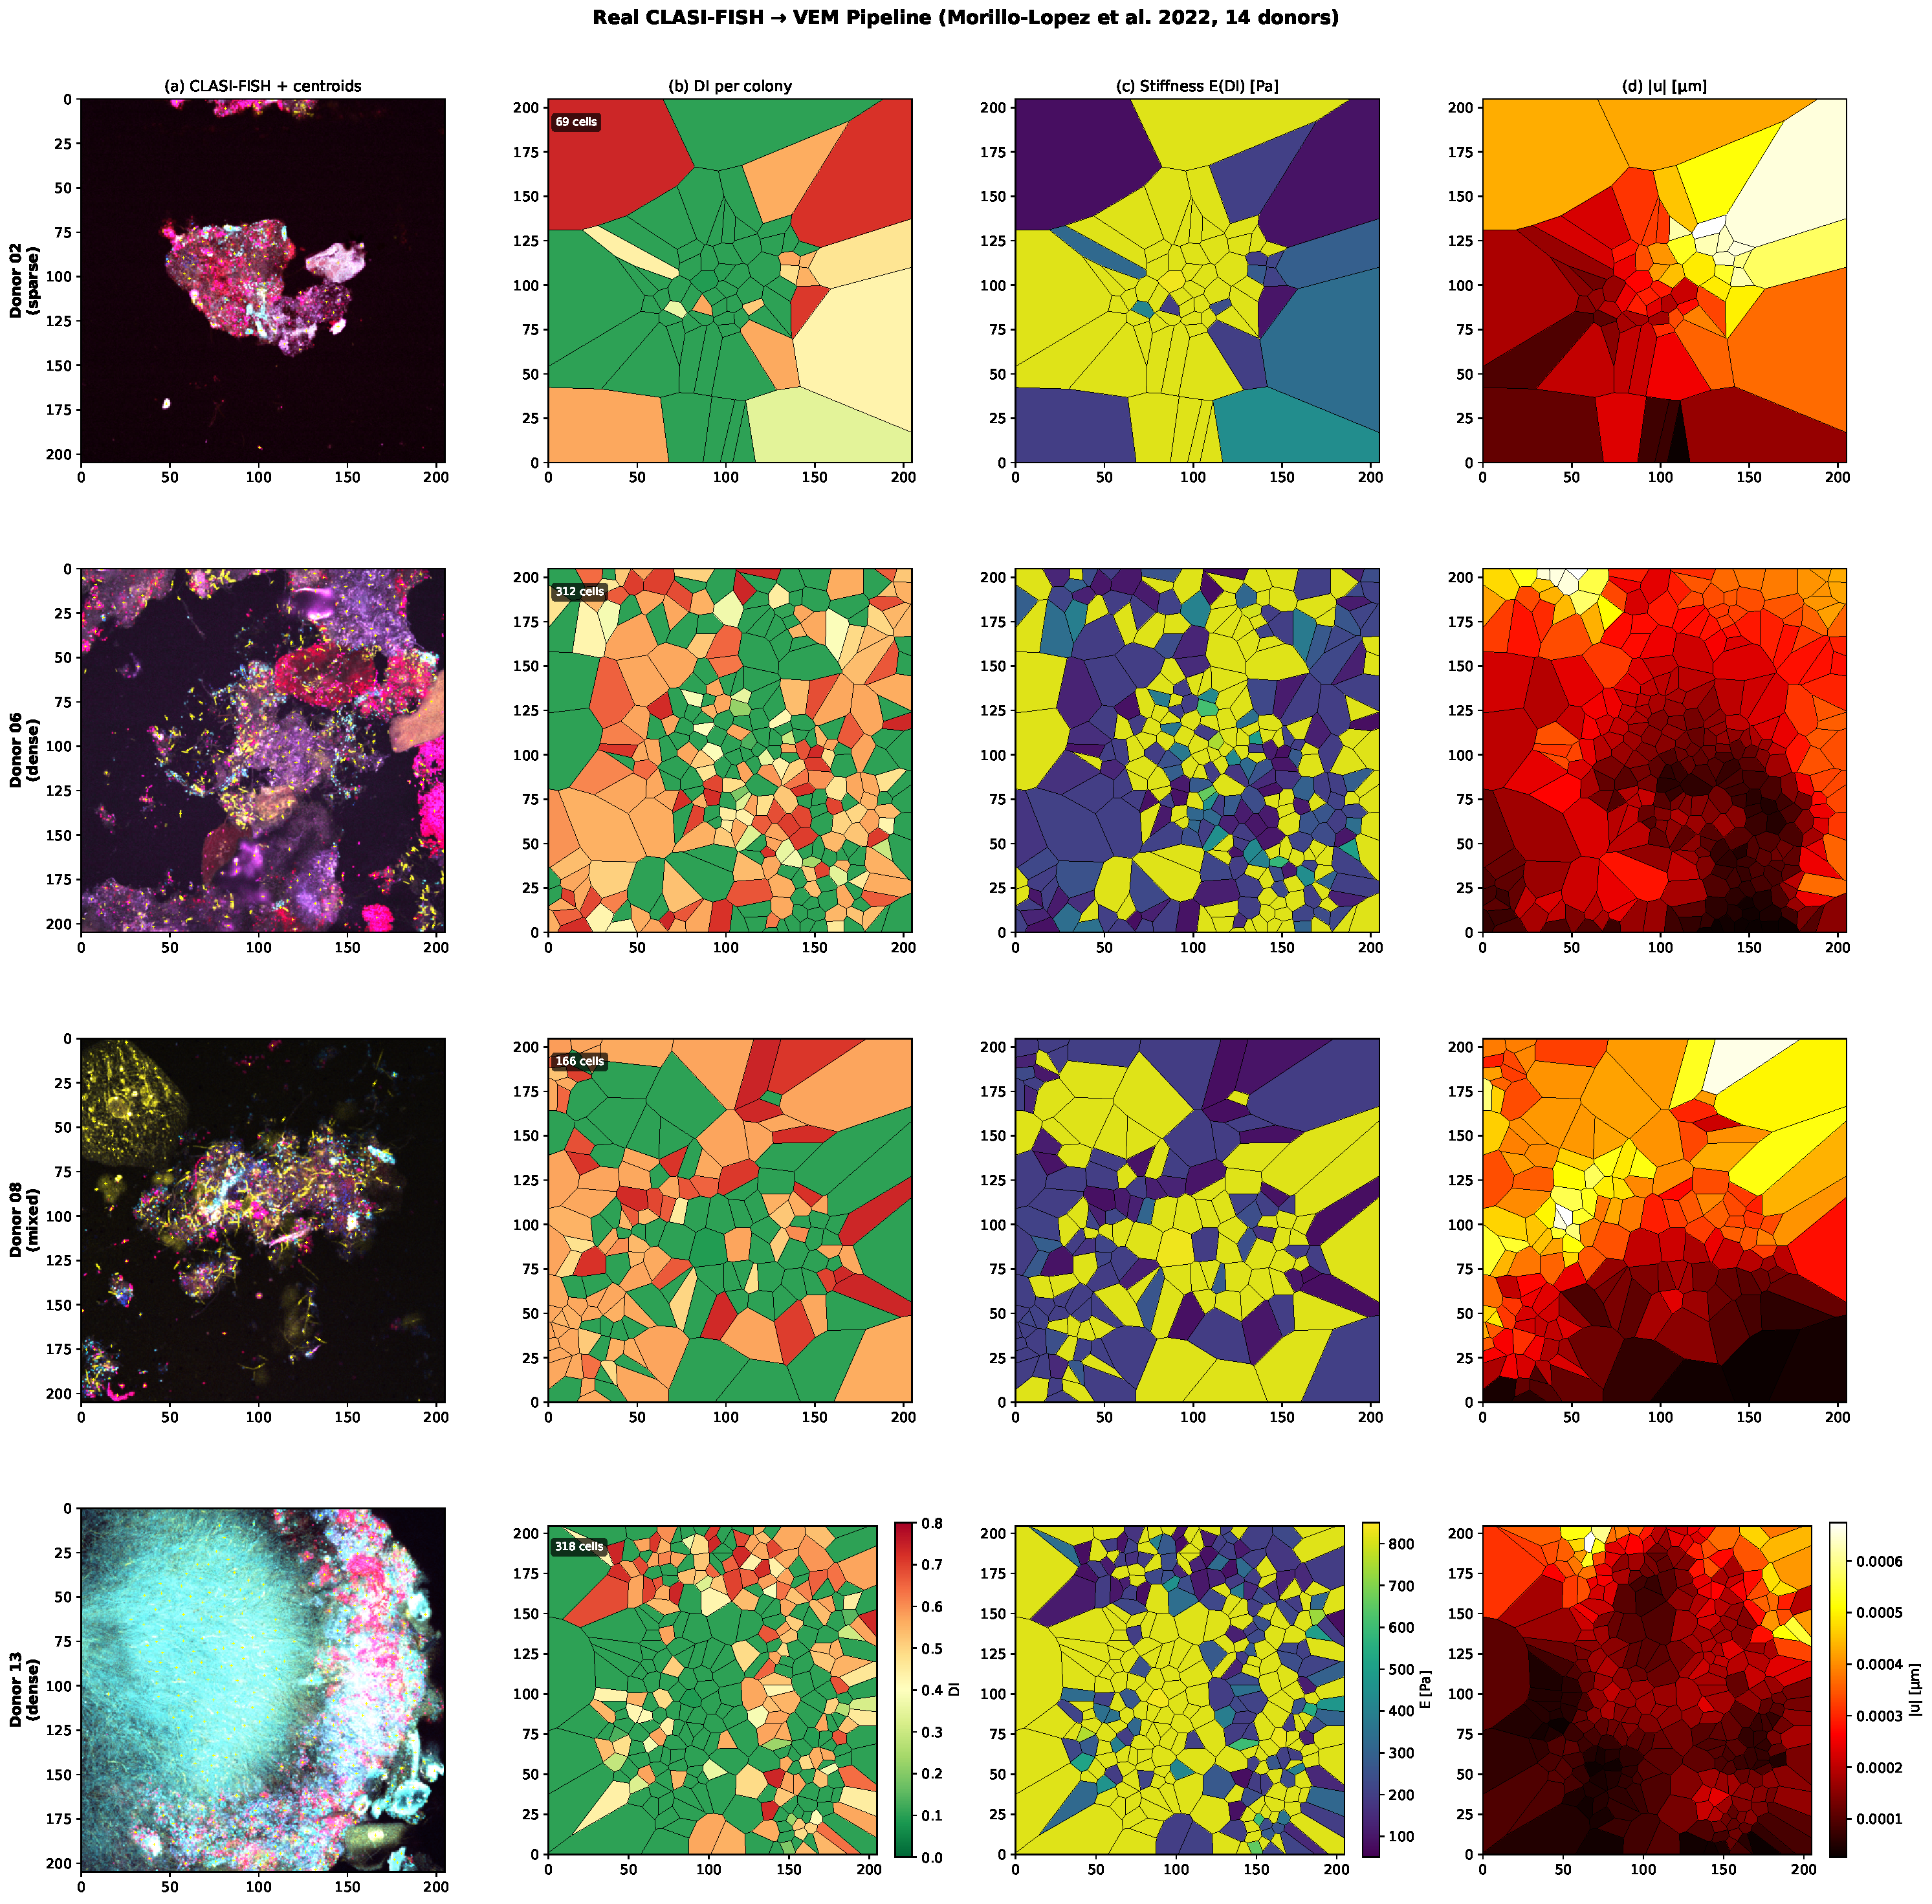
\includegraphics[width=\linewidth]{fig13_confocal_real.pdf}
  \caption{Real CLASI-FISH $\to$ VEM pipeline for 4 representative
  donors~\cite{MorilloLopez2022}. Columns: (a) FISH image with
  detected centroids (yellow), (b) Voronoi mesh coloured by DI,
  (c) stiffness $E(\DI)$, (d) displacement $|\vect{u}|$.
  Colony density varies from 69 (donor~2) to 318 (donor~13).}
  \label{fig:confocal}
\end{figure}

\begin{table}[t]
  \centering
  \caption{Summary of CLASI-FISH $\to$ VEM results across 14 donors.}
  \label{tab:confocal}
  \begin{tabular}{lrrrr}
    \toprule
    Donor & Colonies & DI (mean) & $\bar{E}$ [Pa] & $|\vect{u}|_\mathrm{max}$ [$\mu$m] \\
    \midrule
    02 (sparse) & 69 & 0.21 & 670 & $1.0 \times 10^{-2}$ \\
    06 (dense) & 312 & 0.36 & 467 & $6.9 \times 10^{-3}$ \\
    08 (mixed) & 166 & 0.39 & 437 & $1.1 \times 10^{-2}$ \\
    13 (dense) & 318 & 0.30 & 553 & $9.5 \times 10^{-4}$ \\
    \midrule
    All 14 & 220$\pm$82 & 0.33$\pm$0.05 & 517$\pm$56 & --- \\
    \bottomrule
  \end{tabular}
\end{table}

\subsection{Stress relaxation at different DI levels}

Fig.~\ref{fig:relaxation} shows VE-VEM stress relaxation curves
for three uniform DI levels under confined step strain.
The VEM solutions (solid) match analytical predictions (dashed)
at all DI levels, as expected from Remark~\ref{rem:machprec}.
Higher DI yields lower initial stress (softer material) and
faster relaxation (shorter $\tau$), consistent with
experimental observations that EPS-rich biofilms exhibit
longer relaxation times~\cite{Peterson2015,Stoodley1999}.

\begin{figure}[t]
  \centering
  
\includegraphics[width=0.85\linewidth]{fig14_relaxation.pdf}
  \caption{VE-VEM stress relaxation for DI~$= 0.1$, 0.4, 0.8.
  Solid: VEM; dashed: analytical. Vertical dotted lines mark
  $\tau$ for each DI level.}
  \label{fig:relaxation}
\end{figure}

\subsection{CNN-accelerated pipeline: confocal $\to$ DI $\to$ displacement}
\label{sec:ml-pipeline}

The colony-detection and Voronoi meshing steps in
Section~\ref{sec:pipeline} are deterministic image-processing routines
that can be replaced by a trained neural network.
We train a standard U-Net~\cite{Ronneberger2015} ($\approx 7.8$\,M parameters)
on 256$\times$256 patches extracted from all 239 CLASI-FISH images
(14 donors, $\approx 30\,000$ patches after augmentation):
\begin{itemize}[nosep]
  \item \emph{Input}: 3-channel RGB confocal image (normalised to $[0,1]$).
  \item \emph{Output}: pixel-wise $\DI(x,y)$ map.
  \item \emph{Loss}: MSE $+$ $0.2\,\times$ SSIM $+$ $0.1\,\times$
    gradient penalty (promotes spatially smooth predictions).
\end{itemize}
Leave-two-donors-out cross-validation (donors 13 and 14 held out)
yields a mean absolute error $\mathrm{MAE} < 0.05$
across all validation patches (Fig.~\ref{fig:unet-di}).

\begin{figure}[t]
  \centering
  \includegraphics[width=\linewidth]{fig_ml_unet_di_prediction.pdf}
  \caption{U-Net DI prediction on held-out donors.
  Row 1: confocal input; row 2: ground-truth DI from colony detection;
  row 3: U-Net prediction; row 4: absolute error map.}
  \label{fig:unet-di}
\end{figure}

A second CNN (encoder--decoder, $\approx 1.2$\,M parameters) is
trained as a VEM surrogate: given a DI map, it predicts the
displacement magnitude field $|\vect{u}(x,y)|$ that the VEM solver
would produce under the standard GCF loading
(Section~\ref{sec:growth-coupled}).
Training data consist of 500 random spatially-correlated DI fields
solved by the VEM elasticity module.

\paragraph{End-to-end pipeline.}
Chaining the two networks yields a fully differentiable mapping
\[
  \text{confocal image} \;\xrightarrow{\text{U-Net}}\;
  \DI(x,y) \;\xrightarrow{E(\DI)}\;
  E(x,y) \;\xrightarrow{\text{Surrogate}}\;
  |\vect{u}(x,y)|
\]
that runs in $<0.1$\,s on CPU---more than $100\times$ faster than the
traditional colony-detection $\to$ Voronoi $\to$ VEM-solve pipeline
($\approx 10$\,s).
Fig.~\ref{fig:ml-comparison} compares the two pipelines on an unseen
donor~14 image.

\begin{figure}[t]
  \centering
  \includegraphics[width=\linewidth]{fig_ml_e2e_comparison.pdf}
  \caption{Traditional VEM pipeline (top) vs.\ CNN pipeline (bottom)
  for an unseen donor~14 CLASI-FISH image.
  The ML pipeline reproduces the DI pattern and displacement field
  at $> 100\times$ speedup.}
  \label{fig:ml-comparison}
\end{figure}

% =====================================================================
\section{Discussion}
\label{sec:discussion}

\subsection{VEM advantages and limitations for biofilm mechanics}

The 2-step pipeline (colony detection $\to$ Voronoi $\to$ VEM)
eliminates the mesh generation bottleneck that dominates
image-based FEM workflows.
The per-step VEM solve is approximately 1.4$\times$ slower than FEM
due to projection and stabilisation overhead; for problems where
meshing cost is negligible (e.g., structured domains), FEM remains
more efficient.
However, for image-based biofilm problems, the meshing stage
dominates the total pipeline cost, and the VEM pipeline's
near-instant Voronoi tessellation provides a significant advantage.

The VEM convergence rates on Voronoi meshes ($L^2 = 2.16$,
$H^1 = 1.31$) are competitive with FEM on structured triangulations
($L^2 = 1.88$, $H^1 = 0.99$).
The superconvergent $H^1$ rate on Voronoi meshes degrades on
distorted meshes (Section~\ref{sec:nonuniform}), and the stabilisation
parameter $\alpha_s$ has negligible effect for
$\alpha_s \in [0.1, 1.0]$ (Section~\ref{sec:alpha_s}).

Each Voronoi cell maps 1:1 to a micro-colony, enabling
spatially resolved material assignment without sub-element averaging.
However, this 1:1 mapping assumes that colony boundaries align with
Voronoi cell boundaries, which may not hold for irregularly shaped
colonies.

\subsection{Viscoelastic VEM}

The combination of the Simo~\cite{Simo1987} exponential integrator
with VEM is, to our knowledge, novel in the literature, although
inelastic VEM formulations have been developed for
plasticity~\cite{Artioli2017,Wriggers2019}.
The machine-precision result for uniform strain
(Remark~\ref{rem:machprec}) confirms implementation correctness,
while the $h$-convergence study on non-uniform manufactured
solutions (Table~\ref{tab:convergence}) demonstrates that VEM
achieves convergence rates competitive with FEM.

The growth-coupled simulations reveal a \emph{mechanical
bifurcation}: commensal biofilms stiffen over time while dysbiotic
biofilms soften, even starting from comparable initial DI.
This has direct clinical implications: a stiffening biofilm is
harder to remove mechanically, while a softening biofilm may
detach spontaneously under shear~\cite{Stoodley1999}.
The magnitude of this bifurcation depends on the assumed $\tau(\DI)$
relationship (level-C support), and experimental validation with
time-resolved rheometry would strengthen these predictions.

\subsection{Phase-field and cohesive fracture on VEM}

The extension of Aldakheel et al.'s~\cite{Aldakheel2018}
phase-field framework to DI-dependent fracture toughness
enables prediction of composition-dependent crack paths.
The adaptive $h$-refinement capability ($40 \to 121$ cells
over 3 levels, 68\% error reduction) concentrates computational
resources at the crack tip.
The complementary CZM approach is particularly suited for
tooth--biofilm interface failure, where the debonding path is
known \emph{a priori}.
Both fracture models rely on level-C constitutive assumptions
(Table~\ref{tab:support}), so the results should be interpreted
as qualitative predictions of the failure mode rather than
quantitative predictions of critical loads.

\subsection{CNN-accelerated pipeline}

The U-Net trained on the 239 CLASI-FISH images replaces the
colony-detection/Voronoi-meshing steps with a single forward pass,
achieving MAE~$< 0.05$ on held-out donors.
Combined with the VEM surrogate CNN, the full confocal-to-displacement
mapping runs in $< 0.1$\,s, compared to $\sim 10$\,s for the
traditional pipeline---a $> 100\times$ speedup.
This makes real-time DI assessment feasible for clinical
chairside monitoring.
The surrogate approach is conceptually similar to the DeepONet
strategy used in our TMCMC framework~\cite{Klempt2024} for
accelerating forward model evaluation, but here applied to the
spatial (PDE) domain rather than the temporal (ODE) domain.

A key limitation is that the training data are generated by the
colony-detection algorithm itself, so the CNN cannot outperform
the upstream ground-truth quality.
Fine-tuning on manually annotated confocal images or
higher-multiplexed data (HiPR-FISH) could improve accuracy.

\subsection{Limitations}

\begin{enumerate}[nosep]
  \item The DI-to-mechanics mappings $G_c(\DI)$ and $\tau(\DI)$ are
    modelling assumptions without direct experimental calibration
    (level C in Table~\ref{tab:support}).
    Only $E(\DI)$ has indirect experimental support (level B).
  \item The SLS model uses a single relaxation branch;
    Prony series with multiple branches may better capture
    broadband relaxation spectra~\cite{Peterson2015}.
  \item The confocal pipeline is demonstrated on CLASI-FISH
    images~\cite{MorilloLopez2022} with 3 spectral channels;
    higher-multiplexed imaging (e.g., HiPR-FISH~\cite{Shi2020}
    with 65 genera) would require spectral barcode decoding.
  \item $\nu = 0.45$ is assumed throughout; biofilms may approach
    incompressibility ($\nu \to 0.5$), which could require
    volumetric locking mitigation in VEM~\cite{Chi2017}.
  \item The framework is serial; parallel assembly and
    domain decomposition~\cite{Antonietti2022} would be needed
    for clinically relevant 3D problems.
  \item The CNN surrogate is trained on synthetic VEM solutions;
    its accuracy is bounded by the upstream colony-detection
    ground truth and the diversity of training DI fields.
\end{enumerate}

% =====================================================================
\section{Conclusions}
\label{sec:conclusions}

We have presented a Virtual Element Method framework for biofilm
mechanics that:
\begin{enumerate}[nosep]
  \item Reduces the image-to-mechanics pipeline from 5 steps
    (FEM) to 2 steps (VEM), demonstrated on 239 real CLASI-FISH
    images from 14 donors~\cite{MorilloLopez2022}.
  \item Validates the Simo 1987 exponential integrator on VEM meshes
    for uniform strain (machine precision $1.3 \times 10^{-15}$,
    Remark~\ref{rem:machprec}) and non-uniform manufactured
    solutions ($L^2$ rate~2.16, Table~\ref{tab:convergence}).
  \item Demonstrates growth-coupled viscoelastic VEM revealing
    divergent mechanical evolution: commensal biofilms stiffen
    ($E_\infty$: $392 \to 847$\,Pa) while dysbiotic biofilms soften
    ($E_\infty$: $376 \to 153$\,Pa).
  \item Provides phase-field fracture with DI-dependent $G_c$,
    predicting composition-dependent detachment patterns
    (with explicitly identified modelling assumptions).
  \item Includes 12 solver modules and 129 automated tests
    covering linear, nonlinear, viscoelastic, and fracture
    mechanics on arbitrary polygonal/polyhedral elements.
  \item Introduces a CNN-accelerated pipeline (U-Net + VEM surrogate)
    that predicts DI and displacement fields from raw confocal
    images at $>100\times$ speedup over the traditional
    colony-detection/VEM-solve workflow.
\end{enumerate}
To our knowledge, this is the first application of VEM to
biofilm mechanics, combining the VEM solid mechanics expertise
of IKM Hannover~\cite{Wriggers2024,Aldakheel2018} with
TMCMC-calibrated microbial species dynamics~\cite{Klempt2024}.

\begin{acknowledgements}
The authors gratefully acknowledge the computing resources provided
by the IKM cluster at Leibniz Universit\"at Hannover.
\end{acknowledgements}

\section*{Data availability}

All source code, test suites, and figure generation scripts are
available at
\url{https://github.com/keisuke58/VirtualElementMethods}.

\bibliographystyle{spmpsci}
\bibliography{references}

\end{document}
